%%
% Plantilla de Trabajo
% Modificación de una plantilla de Latex de Frits Wenneker para adaptarla 
% al castellano y a las necesidades de escribir informática y matemáticas.
%
% Editada por: Mario Román
%
% License:
% CC BY-NC-SA 3.0 (http://creativecommons.org/licenses/by-nc-sa/3.0/)
%%

%%%%%%%%%%%%%%%%%%%%
% Short Sectioned Assignment
% LaTeX Template
% Version 1.0 (5/5/12)
%
% This template has been downloaded from:
% http://www.LaTeXTemplates.com
%
% Original author:
% Frits Wenneker (http://www.howtotex.com)
%
% License:
% CC BY-NC-SA 3.0 (http://creativecommons.org/licenses/by-nc-sa/3.0/)
%
%%%%%%%%%%%%%%%%%%%%%

%----------------------------------------------------------------------------------------
%	PAQUETES Y CONFIGURACIÓN DEL DOCUMENTO
%----------------------------------------------------------------------------------------

%% Configuración del papel.
% fourier: Usa la fuente Adobe Utopia. (Comentando la línea usa la fuente normal)
\documentclass[paper=a4, fontsize=11pt, spanish]{scrartcl} 
\usepackage{fourier}

% Centra y formatea los títulos de sección.
% Quita la indentación de párrafos.
\usepackage{sectsty} % Allows customizing section commands
\allsectionsfont{\centering \normalfont\scshape} % Make all sections centered, the default font and small caps
\setlength\parindent{0pt} % Removes all indentation from paragraphs - comment this line for an assignment with lots of text

%% Castellano.
% noquoting: Permite uso de comillas no españolas.
% lcroman: Permite la enumeración con numerales romanos en minúscula.
% fontenc: Usa la fuente completa para que pueda copiarse correctamente del pdf.
\usepackage[spanish,es-noquoting,es-lcroman]{babel}
\usepackage[utf8]{inputenc}
\usepackage[T1]{fontenc}
\selectlanguage{spanish}

% Para incluir imágenes y colocarlas
\usepackage{graphics,graphicx, float, url}

%% Matemáticas.
% Paquetes de la AMS. Para entornos de ecuaciones.
\usepackage{amsmath,amsfonts,amsthm}

% Enlaces
\usepackage[hidelinks]{hyperref}

%----------------------------------------------------------------------------------------
%	TÍTULO
%----------------------------------------------------------------------------------------
% Título con las líneas horizontales, nombres y fecha.

\newcommand{\horrule}[1]{\rule{\linewidth}{#1}} % Create horizontal rule command with 1 argument of height

\title{
  \normalfont \normalsize 
  \textsc{Universidad de Granada.} \\ [25pt] % Your university, school and/or department name(s)
  \horrule{0.5pt} \\[0.4cm] % Thin top horizontal rule
  \huge Ejercicios de Álgebra, Grupos y Representaciones \\ % The assignment title
  \horrule{2pt} \\[0.5cm] % Thick bottom horizontal rule
}

\author{Óscar Bermúdez Garrido} % Your name

\date{\normalsize\today} % Today's date or a custom date

%----------------------------------------------------------------------------------------
%	DOCUMENTO
%----------------------------------------------------------------------------------------


\begin{document}
	\maketitle % Escribe el título
	
	\newpage

	\begin{enumerate}
		% Pág 17
		\item * Consideramos $T: \mathbb{R}^3 \rightarrow \mathbb{R}^3$ una aplicación lineal, y la estructura
		de $\mathbb{R}[X]$-módulo correspondiente sobre $\mathbb{R}^3$. Discutir los posibles valores de la
		longitud de $\mathbb{R}^3$ como $\mathbb{R}$-módulo. Poner un ejemplo de $T$ para el que se alcance
		cada longitud.
		\subsubsection*{Solución}
		Dado que la dimensión de $\mathbb{R}^3$ como espacio vectorial es 3, su longitud será, como máximo, 3.
		
		\begin{itemize}
			\item \textbf{Longitud 1:} $0 \subseteq \mathbb{R}^3$, es decir, sería simple.
			
			Sin embargo, este caso no puede darse pues toda aplicación lineal $T: \mathbb{R}^3 \rightarrow
			\mathbb{R}^3$ nos da una ecuación polinómica de grado 3 con coeficientes reales $|T - \lambda I|
			= 0$ que tiene una solución en los reales. Por tanto, obtenemos así un subespacio estricto que
			queda fijo por $T$, es decir, un submódulo $\Rightarrow$ no es simple.
			
			\item \textbf{Longitud 2:} $0 \subseteq N \subseteq \mathbb{R}^3$
			
			En este caso, necesitamos encontrar una aplicación que mueva un elemento bidimensional mientras
			deja fija otro unideminensional. Por ejemplo, el giro sobre el eje (1, 0, 0):
			
			$$T = \begin{pmatrix}
				1 & 0 & 0 \\
				0 & 0 & 1 \\
				0 & -1 & 0
			\end{pmatrix}$$
			
			Claramente, el subespacio generado por el eje queda fijo por esta acción, así que se tiene que
			$N = <(0, 1, 0), (0, 0, 1)>$.
			
			\item \textbf{Longitud 3:} $0 \subseteq N_1 \subseteq N_2 \subseteq \mathbb{R}^3$
			
			Este caso es el más fácil de todos pues nos baste con tomar $T = I_3$ para tener la descomposicón
			$0 \subseteq <(1, 0, 0)> \subseteq <(1, 0, 0), (0, 1, 0)> \subseteq \mathbb{R}^3$.
		\end{itemize}
		
		% Pág 17
		\item Sea $\mathbb{P}_n$ el espacio vectorial real de las funciones polinómicas en una variable de grado
		menor o igual que $n$. Sea $T: \mathbb{P}_n \rightarrow \mathbb{P}_n$ la aplicación lineal que asigna a
		cada polinomio su derivada. Calcular una serie de composición de $\mathbb{P}_n$ visto como $\mathbb{R}[X]
		-módulo$ vía $T$.
		\subsubsection*{Solución}
		Sabemos que una base del espacio de polinomio de grado menor o igual que $k$ sería $M_k = \{1, \dots, x^k\}$.
		Claramente, podemos ver que $<M_k> = <\{1, \dots, x^k\}>$ es un submódulo de $\mathbb{P}_n$ cerrado para
		la derivada puesto que $M_k$ es base del espacio de polinomios de grado menor o igual que $k$ y, al estar
		en un cuerpo de característica 0, su derivada es de grado menor o igual que $k-1$ y claramente $M_{k-1}
		\subseteq <M_k>$.
		
		Además, dado que $M_k = <x^k> M_k/_{M_{k-1}}$ se tiene que $M_k$ es de dimensión 1 en el cuerpo de los
		reales sobre $M_k/_{M_{k-1}}$ y por tanto simple.
		
		Así formaríamos la serie de descomposición: $0 \subset <M_1> \subset <M_2> \subset \dots \subset <M_n> =
		\mathbb{P}_n$.
		
		% Pág 17
		\item ** En las condiciones del ejercicio anterior, calcular todos los $\mathbb{R}$-submódulos de
		$\mathbb{P}_n$.
		\subsubsection*{Solución}
		En el ejercicio anterior vimos los módulos de la forma $<M_k>$, que eran los que formaban la serie de
		descomposición que dimos. Veamos ahora que estos son los únicos submódulos de $\mathbb{P}_n$.
		
		Supongamos que existen más submódulos de $\mathbb{P}_n$, entonces tomemos un polinomio $p(x) = x^k +
		a_{k-1}x^{k-1} + \cdots + a_1x+a_0$ con $k \leq n \Rightarrow p(x) \in \mathbb{P}_n$ y sea $N_p$ el menor
		submódulo tal que $p(x) \in N_p$.
		
		Como $N_p$ es un submódulo debe ser cerrado para $T$, luego se tiene
		que $\delta p(x) = kx^{k-1} + (k-1)a_{k-1}x^{k-2} + \cdots + 2a_2x+a_1 \in N_p$ y análogamente se deduce
		que$\delta^2 p(x), \dots, \delta^{k} \in N_p$, es decir, $<\{p, \delta p, \delta^2 p, \dots, \delta^k p\}>
		\subseteq N_p$.
		
		Entonces, es inmediato comprobar que $ <M_k> \cong <\{p, \delta p, \delta^2 p, \dots, \delta^k p\}>$, y
		se tiene que $<M_k> \subseteq N_p$ pero por cómo hemos definido $N_p$ se deduce que $<M_k> = N_p$.
		
		% Pág 19
		\item ** Supongamos $T: V \rightarrow V$ un endomorfismo $K$-lineal, donde $V$ es un espacio vectorial de
		dimensión finita que consideramos, como de costumbre, como un $K$-módulo. Supongamos que el polinomio
		mínimo $m(X)$ de $T$ es irreducible en $K[X]$. Demostrar que existen $K[X]$-submódulos simples $V_1, \dots,
		V_t$ de $V$ tal que $V = V_1 \bigoplus \dots \bigoplus V_t$ como $K$-módulo.
		\subsubsection*{Solución}
		Dado que el polinomio mínimo $m(X)$ es irreducible $\Rightarrow$ el ideal $(m(X))$ es maximal, por tanto,
		se tiene que el cociente $K[X]/_{(m(X))}$ es un cuerpo que también denotaremos $F$.
		
		Como tenemos que $K[X] \rightarrow End_K(V)$, al aplicarle el Primer Teorema de Isomorfía, podemos
		descomponerlo como $K[X] \rightarrow K[X]/_{(m(X))} \hookrightarrow End_K(V)$, de lo que se concluye que
		$V$ es $F$-espacio vectorial.
		
		Ahora, dado que $V$ tiene una base finita como $K$-espacio vectorial y que $K \subseteq F$, tenemos que
		$V$ tiene un sistema de generadores finito como $F$-espacio vectorial del que, en virtud de un corolario
		visto en clase, podemos extraer un subconjunto $\{V_1, V_2, \dots, V_t\}$que genere una base, esto es,
		$V = V_1 \bigoplus V_2 \bigoplus \dots \bigoplus V_t$.
		
		Finalmente, por la forma de construcción de esta base, tenemos que sus elementos son isomorfos a $F$ y,
		por tanto, $K[X]$-submódulos simples.
		
		% Pág 19
		\item ** En las condiciones del ejercicio anterior, demostrar que el polinomio característico de $T$ es
		$m(X)^t$.
		\subsubsection*{Solución}
		Empecemos porque $T$ debe satisfacer su ecuación característica por el Teorema de Cayley-Hamilton, y
		como $m(X)$ es un divisor de todo polinomio $p(X)$ que cumpla $T$, en particular, $m(X)$ es un divisor
		del polinomio característico de $T$.
		
		Veamos ahora que no sólo $m(X)$ divide al polinomio característico sino que es su único factor
		irreducible, esto es, el polinomio característico de $T$ es de la forma $(m(X))^n$ para algún $n \in
		\mathbb{N}$.
		
		Sea el polinomio $p(X)$ un factor irreducible del polinomio característico, entonces se tiene que
		tiene una raíz $\alpha$ en la clausura algebraica de $K$. Esto equivale a tener un vector propio
		$\lambda$ con coeficientes en la clausura de $K$ cumpliendo $T\lambda = \alpha\lambda$.
		
		Aplicando el polinomio mínimo al vector, tenemos que $0 = m(T)\lambda = m(\alpha)\lambda \Rightarrow
		\alpha$ es una raíz en la clausura algebraica de $m(X)$. Por tanto, $p(X)$ es un factor irreducible
		de $m(X)$, que también es irreducible, lo que nos lleva a que $m(X) = p(X) \Rightarrow$ el polinomio
		característico de $T$ sólo tiene a $m(X)$ como único factor irreducible, es decir, es de la forma
		$(m(X))^n$.
		
		Por último, como el grado del polinomio característico tiene el mismo valor que la dimensión del
		espacio en que se genera, calcularemos la $dim_K(V)$. Por la construcción que hicimos de $V$ con
		$V_1, V_2, \dots, V_t$ y que $V_i \cong F = K[X]/_{(m(X))} \Rightarrow dim_K(V) = t \cdot dim_K (V_i)
		= t \cdot dim_K(F) = t \cdot gr(m(X)) \Rightarrow (m(X))^t$ es el polinomio característico.
		
		% Pág 22
		\item ** Sea $R$ un álgebra sobre un cuerpo de característica distinta de 2, y $a, b, e \in R$ idempotentes.
		Demostrar que si $e = a + b$, entonces $ab = ba = 0$. Si la característica es 2, encontrar un contraejemplo
		con $a \neq b$.
		\subsubsection*{Solución}
		Si $e = a+b$ tenemos que $e^2 = (a+b)^2 = a^2 + b^2 + ab + ba = a + b + ab + ba = a+b \Rightarrow ab + ba
		= 0 \Rightarrow ba = -ab \Leftrightarrow ab = -ba$ y volviendo a utilizar que $a$ y $b$ son idempotentes,
		se llega a que $ab = a^2b = a(-ba) = -aba = (-ab)a = ba^2 = ba \Rightarrow 2ab = 2ba = ab + ba = 0$ pero
		como la característica del cuerpo no es 2, la única posibilidad es que $ab = ba = 0$.
		
		Como contraejemplo, nos iremos al álgebra $M_2(\mathbb{F}_2)$ y tomaremos $a = I_2$, $\displaystyle b =
		\begin{pmatrix} 1 & 0 \\ 0 & 0 \end{pmatrix}$, entonces $\displaystyle e = a+b = \begin{pmatrix} 0 & 0
		\\ 0 & 1 \end{pmatrix}$, claramente todas son idempotentes pero $ab = ba = b \neq 0_{2,2}$.
	
		% Pág 31
		\item * Calcular explícitamente una representación real no trivial de grado 2 del grupo de permutaciones
		$S_3$.
		\subsubsection*{Solución}
		Representaremos el grupo de las permutaciones $S_3$ como las aplicaciones sobre $\mathbb{R}^2$ que dejan
		invariantes los vértices de un triángulo equilátero como el de la imagen:
		
		\begin{figure}[H]
			\centering
			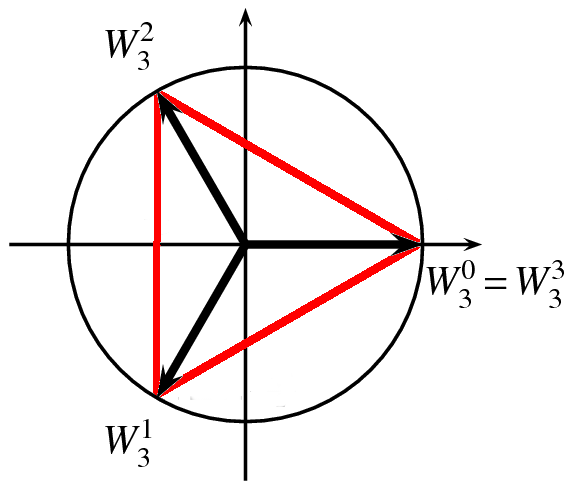
\includegraphics[width=5cm]{./3rd-roots-of-unity.png}
			\caption{Raíces cúbicas de la unidad. Imagen retocada de
			\href{https://upload.wikimedia.org/wikipedia/commons/3/3a/3rd-roots-of-unity.png}{Wikipedia}}
		\end{figure}
		
		En particular, tomaremos $A = W_3^0 = (0, 1)$, $\displaystyle B = W_3^2 = \left(\frac{-1}{2},
		\frac{\sqrt{3}}{2}\right)$ y $\displaystyle C = W_3^1 = \left(\frac{-1}{2}, \frac{-\sqrt{3}}{2}\right)$.
		Además, tomaremos $b=\{A, B\}$ como base de $\mathbb{R}^2$ notando que $C = -(A+B)$.
		
		Visto esto, nos basta ver que $A =_b (1, 0)$, $B =_b (0, 1)$ y $C =_b (-1, -1)$ y luego se calculan las
		operaciones de $\phi: S_3 \rightarrow GL\left(\mathbb{R}^2\right)$ como:
		$$\left.\begin{aligned}
			(1\ 2)A = A\\
			(1\ 2)B = B
		\end{aligned}\right\} \Rightarrow\phi(id) = \begin{pmatrix} 1 & 0\\ 0 & 1 \end{pmatrix}$$
		
		$$\left.\begin{aligned}
			(1\ 2)A = B\\
			(1\ 2)B = A
		\end{aligned}\right\} \Rightarrow \phi((1\ 2)) = \begin{pmatrix} 0 & 1\\ 1 & 0 \end{pmatrix}$$
		
		$$\left.\begin{aligned}
			(1\ 3)A = C\\
			(1\ 3)B = B
		\end{aligned}\right\} \Rightarrow \phi((1\ 3)) = \begin{pmatrix} -1 & 0\\ -1 & 1 \end{pmatrix}$$
		
		$$\left.\begin{aligned}
			(2\ 3)A = A\\
			(2\ 3)B = C
		\end{aligned}\right\} \Rightarrow \phi((2\ 3)) = \begin{pmatrix} 1 & -1\\ 0 & -1 \end{pmatrix}$$
		
		$$\left.\begin{aligned}
			(1\ 2\ 3)A = B\\
			(1\ 2\ 3)B = C
		\end{aligned}\right\} \Rightarrow \phi((1\ 2\ 3)) = \begin{pmatrix} 0 & -1\\ 1 & -1 \end{pmatrix}$$
		
		$$\left.\begin{aligned}
			(1\ 3\ 2)A = C\\
			(1\ 3\ 2)B = A
		\end{aligned}\right\} \Rightarrow \phi((1\ 3\ 2)) = \begin{pmatrix} -1 & 1\\ -1 & 0 \end{pmatrix}$$
		
       
		% Pág 43
		\item Si $r \in \mathbb{Q}$ es un entero algebraico, entonces $r \in \mathbb{Z}$\footnote{En el enunciado
		original, era una $q$ pero por conveniencia de notación, la he cambiado.}.
		\subsubsection*{Solución}
		Supongamos que $r$ es un entero algebraico pero $r \notin \mathbb{Z}$ y sea $f(x) = x^n + a_{n-1}x^{n-1}
		+ \dots + a_1x + a_0$ con $a_{n-1}, \dots, a_1, a_0 \in \mathbb{Z}$ el polinomio de coeficientes enteros
		del que $r$ es raíz, esto es, $f(r) = 0$.
		
		Como $r \in \mathbb{Q}$ podemos expresarlo como $\displaystyle r = \frac{p}{q}$ con $(p, q) = 1$, entonces
		nos queda que $\displaystyle f(r) = f\left(\frac{p}{q}\right) = \left(\frac{p}{q}\right)^n + a_{n-1}
		\left(\frac{p}{q}\right)^{n-1} + \dots + a_1\frac{p}{q} + a_0 = 0$.
		
		Después, multiplicamos toda la expresión por $q^n$ para quitarnos los denominadores: $p^n + a_{n-1}qp^{n-1}
		+ \dots + a_1q^{n-1}p + a_0q^n = 0$
		
		Llegados a este punto, vemos que $-p^n = q \cdot \left(a_{n-1}p^{n-1} + \dots + a_1q^{n-2}p + a_0q^{n-1}\right)
		\Rightarrow q$ divide a $p^n$ pero recordemos que $(p, q) = 1$.
	\end{enumerate}
\end{document}
